%----------------------------------------------------------------------------------------
% Parallel histogram generation using OpenMP
%----------------------------------------------------------------------------------------

\section{Parallel histogram generation using OpenMP}

\subsection{Compile and run the template code with a single thread to verify
that the serial version is correct}

\Cref{fig:lab3part3a} shows the terminal output for the execution of the template
code with one thread. 

\begin{figure}[ht]
	\centering
	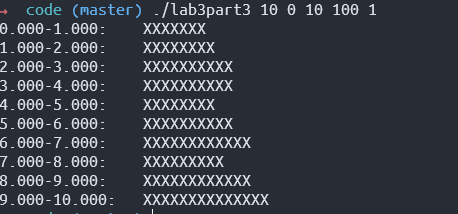
\includegraphics[width=\textwidth]{graphics/P3_a_terminal_output.PNG}
	\caption{Terminal output for execution with a single thread, using a 
	data range bewteeen 0 and 10, a total of 100 data points, and 10 equally
	spaced bins}
	\label{fig:lab3part3a}
\end{figure}

\subsection{Parallelize the code for multi-thread execution by ONLY adding OpenMP
directives}

\Cref{lst:lab3part3a} shows the changes within the template code to parallelize
by only adding OpenMP directives.

\vspace{0.5cm}
\lstinputlisting[
	style=CStyle,
	firstline=95, % First line of code
	lastline=119, % Lastl ine of code
	caption=Parallizing the code for multi-threaded execution (line 92-116 in lab3part3.c), % Caption above the listing
	label=lst:lab3part3a, % Label for referencing this listing
	frame=single, % Frame around the code listing
	showstringspaces=false, % Don't put marks in string spaces
	numbers=left, % Line numbers on left
	numberstyle=\normalsize % Line numbers styling
	]{../code/lab3part3.c}

\subsubsection{Explain how your code achieves parallelization.}

The first OpenMP directive is initializing the parallel environment
within the code block from line 3 to 25 in \cref{lst:lab3part3a}. This
directive will create a team of threads equal to the thread count specified
by the user, and all variables within that environment are within their own
scope in each thread (I.E stored within the stack of each thread).

The next directive divides the work of determining which data point falls
under which bin amongst the threads. It outputs the frequency of data point 
to a local histrogram counter in a form of an array. Here, the variable \emph{bin} must be 
declared private which makes a separte copy into each thread's stack. This is
done because we want to avoid race conditions for when multiple thread tries
to write to \emph{bin} at the same time.

The third and final \emph{for} directive sum up the local histogram counter
to the final output histogram. Here a nested for loop is used, because it needs
to iterate over each local histogram, and then each bin within the local histogram
to sum up the total histogram count.

\subsubsection{Describe at what points new threads are forked and joined and
which part of the code are executed by which threads.}

New threads are forked when the parallel environment begins (line 2 in 
\cref{lst:lab3part3a}) and they are joined once the parallel environment ends
(line 25 \cref{lst:lab3part3a}). Within the parallel environment, work
are divided amongst the threads, I.E, through the use of the \emph{for} pragma.
Any code outside of the parallel environment are run in serial by the main thread.

\subsection{Tabulate the speedup and efficiency for 1,2,4,8 threads using a data
range between 0 and 10, a total of $10^7$ data points, and 10 equally spaced bins}

\begin{center}
\begin{tabular}{|| c | c | c | c ||}
	\hline
	Threads & Time (s) & Speedup & Efficiency (\%) \\ [0.5ex]
	\hline 
	1 & 0.474 & N/A & 100 \\
	2 & 0.295 & 1.607 & 80.34 \\
	4 & 0.227 & 2.088 & 52.20 \\
	8 & 0.195 & 2.431 & 30.38\\
	\hline
\end{tabular}
\end{center}

\begin{figure}[ht]
	\centering
	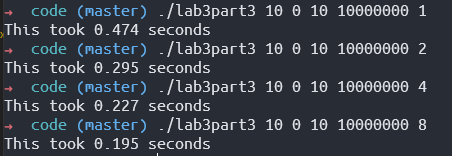
\includegraphics[width=\textwidth]{graphics/P3_c_terminal_output.PNG}
	\caption{Terminal output for execution with 1, 2, 4, 8 threads respectively,
	using a data range bewteeen 0 and 10, a total of $10^7$ data points, and 10 equally
	spaced bins.}
	\label{fig:lab3part3c}
\end{figure}